\begin{frame}{What is \texttt{oSCR}?}

The \textcolor{mLightBrown}{\texttt{o}} is for \emph{open}

\begin{itemize}
\item<1->  built upon various functions in \texttt{scrbook}  
\item<2-> an editable and evolving code base
\item<3->  a community of contributors  
  \begin{itemize}
  \item<3-> \textcolor{gray}{\textit{contributing}} ideas
  \item<3-> \textcolor{gray}{\textit{contributing}} problems
  \item<3-> \textcolor{gray}{\textit{contributing}} solutions
  \item<3-> \textcolor{gray}{\textit{contributing}} code
  \end{itemize}
\item<4-> a philosophy of 'parallel publishing' 
  \begin{itemize}
  \item<4-> increase transparency
  \item<4-> increase accessibility
  \end{itemize}
\end{itemize}

\begin{tikzpicture}[overlay]
\node[inner sep=0pt] (one) at (10,1) {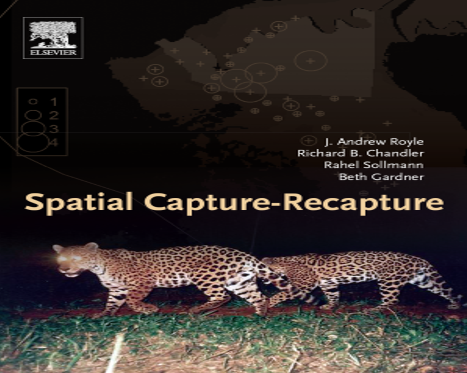
\includegraphics[height=1.2in]{scrbook.png}};
\end{tikzpicture}

\end{frame}

\begin{frame}[fragile]{\texttt{oSCR} - Data organization and structure}

The \texttt{scrFrame} is the main data object containing the essentials
for model fitting:

\scriptsize

\begin{Shaded}
\begin{Highlighting}[]
\NormalTok{sf <-}\StringTok{ }\KeywordTok{make.scrFrame}\NormalTok{(caphist,       }\CommentTok{# spatial encounter histories}
                    \NormalTok{traps,         }\CommentTok{# trap coordinates}
                    \NormalTok{trapCovs,      }\CommentTok{# trap level covariates}
                    \NormalTok{indCovs,       }\CommentTok{# sex data}
                    \NormalTok{trapOperation, }\CommentTok{# binary operation indicator}
                    \NormalTok{type           }\CommentTok{# data format type**}
                    \NormalTok{)}
\end{Highlighting}
\end{Shaded}

\normalsize

\texttt{caphist}:

\end{frame}

\begin{frame}[fragile]{\texttt{oSCR} - Data organization and structure}

The \texttt{scrFrame} is the main data object containing the essentials
for model fitting:

\scriptsize

\begin{Shaded}
\begin{Highlighting}[]
\NormalTok{sf <-}\StringTok{ }\KeywordTok{make.scrFrame}\NormalTok{(caphist,       }\CommentTok{# spatial encounter histories}
                    \NormalTok{traps,         }\CommentTok{# trap coordinates}
                    \NormalTok{trapCovs,      }\CommentTok{# trap level covariates}
                    \NormalTok{indCovs,       }\CommentTok{# sex data}
                    \NormalTok{trapOperation, }\CommentTok{# binary operation indicator}
                    \NormalTok{type           }\CommentTok{# data format type**}
                    \NormalTok{)}
\end{Highlighting}
\end{Shaded}

\normalsize

\texttt{traps}:

\end{frame}

\begin{frame}[fragile]{\texttt{oSCR} - Data organization and structure}

The \texttt{scrFrame} is the main data object containing the essentials
for model fitting:

\scriptsize

\begin{Shaded}
\begin{Highlighting}[]
\NormalTok{sf <-}\StringTok{ }\KeywordTok{make.scrFrame}\NormalTok{(caphist,       }\CommentTok{# spatial encounter histories}
                    \NormalTok{traps,         }\CommentTok{# trap coordinates}
                    \NormalTok{trapCovs,      }\CommentTok{# trap level covariates}
                    \NormalTok{indCovs,       }\CommentTok{# sex data}
                    \NormalTok{trapOperation, }\CommentTok{# binary operation indicator}
                    \NormalTok{type           }\CommentTok{# data format type**}
                    \NormalTok{)}
\end{Highlighting}
\end{Shaded}

\normalsize

\texttt{trapCovs}:

\end{frame}

\begin{frame}[fragile]{\texttt{oSCR} - Data organization and structure}

The \texttt{scrFrame} is the main data object containing the essentials
for model fitting:

\scriptsize

\begin{Shaded}
\begin{Highlighting}[]
\NormalTok{sf <-}\StringTok{ }\KeywordTok{make.scrFrame}\NormalTok{(caphist,       }\CommentTok{# spatial encounter histories}
                    \NormalTok{traps,         }\CommentTok{# trap coordinates}
                    \NormalTok{trapCovs,      }\CommentTok{# trap level covariates}
                    \NormalTok{indCovs,       }\CommentTok{# sex data}
                    \NormalTok{trapOperation, }\CommentTok{# binary operation indicator}
                    \NormalTok{type           }\CommentTok{# data format type**}
                    \NormalTok{)}
\end{Highlighting}
\end{Shaded}

\normalsize

\texttt{indCovs}:

\end{frame}

\begin{frame}[fragile]{\texttt{oSCR} - Data organization and structure}

The \texttt{scrFrame} is the main data object containing the essentials
for model fitting:

\scriptsize

\begin{Shaded}
\begin{Highlighting}[]
\NormalTok{sf <-}\StringTok{ }\KeywordTok{make.scrFrame}\NormalTok{(caphist,       }\CommentTok{# spatial encounter histories}
                    \NormalTok{traps,         }\CommentTok{# trap coordinates}
                    \NormalTok{trapCovs,      }\CommentTok{# trap level covariates}
                    \NormalTok{indCovs,       }\CommentTok{# sex data}
                    \NormalTok{trapOperation, }\CommentTok{# binary operation indicator}
                    \NormalTok{type           }\CommentTok{# data format type**}
                    \NormalTok{)}
\end{Highlighting}
\end{Shaded}

\normalsize

\texttt{trapOperation}:

\end{frame}

\begin{frame}[fragile]{\texttt{oSCR} - Data organization and structure}

The \texttt{scrFrame} is the main data object containing the essentials
for model fitting:

\scriptsize

\begin{Shaded}
\begin{Highlighting}[]
\NormalTok{sf <-}\StringTok{ }\KeywordTok{make.scrFrame}\NormalTok{(caphist,       }\CommentTok{# spatial encounter histories}
                    \NormalTok{traps,         }\CommentTok{# trap coordinates}
                    \NormalTok{trapCovs,      }\CommentTok{# trap level covariates}
                    \NormalTok{indCovs,       }\CommentTok{# sex data}
                    \NormalTok{trapOperation, }\CommentTok{# binary operation indicator}
                    \NormalTok{type           }\CommentTok{# data format type**}
                    \NormalTok{)}
\end{Highlighting}
\end{Shaded}

\normalsize

\texttt{type}:

\end{frame}

\begin{frame}{\texttt{oSCR} - Data summaries}

\begin{itemize}[<+->]
\tightlist
\item
  something
\end{itemize}

\end{frame}

\begin{frame}{\texttt{oSCR} - Model fitting}

\begin{itemize}[<+->]
\tightlist
\item
  oSCR.fit()
\item
  multi-session (\textasciitilde{}session)
\item
  sex-structured models (\textasciitilde{}sex)
\end{itemize}

\end{frame}

\begin{frame}{\texttt{oSCR} - Model output}

\end{frame}

\begin{frame}{\texttt{oSCR} - Model selection}

\begin{itemize}[<+->]
\tightlist
\item
  fitList.oSCR()
\item
  modSel.oSCR()
\item
  ma.coef()
\end{itemize}

\end{frame}

\begin{frame}{Exercise: Ocelot data}

\begin{itemize}[<+->]
\tightlist
\item
  load
\item
  format
\item
  fit
\end{itemize}

Additional oSCR topics {[}time permitting - can be squeezed out{]}
making things run faster with starting values state space buffer state
space resolution trimming the state space plotting the output

\end{frame}

\begin{frame}[fragile]{What is a fucking histogram?}

This is a fucking histogram:

\begin{itemize}[<+->]
\tightlist
\item
  level 1

  \begin{itemize}[<+->]
  \tightlist
  \item
    level 2

    \begin{itemize}[<+->]
    \tightlist
    \item
      level 3 normalsize
    \end{itemize}
  \end{itemize}
\end{itemize}

\begin{Shaded}
\begin{Highlighting}[]
\KeywordTok{hist}\NormalTok{(}\KeywordTok{rnorm}\NormalTok{(}\DecValTok{1000}\NormalTok{))}
\end{Highlighting}
\end{Shaded}

\includegraphics{oSCR_files/figure-beamer/unnamed-chunk-8-1.pdf}

\end{frame}

\begin{frame}[fragile]{What does code look like?}

Code \emph{looks} \textbf{like} \texttt{this}:

normalsize

\begin{Shaded}
\begin{Highlighting}[]
\NormalTok{M <-}\StringTok{ }\DecValTok{250} \CommentTok{# Number of sites}
\NormalTok{J <-}\StringTok{ }\DecValTok{3} \CommentTok{# num secondary sample periods}
\NormalTok{T <-}\StringTok{ }\DecValTok{10} \CommentTok{# num primary sample periods}
\NormalTok{psi <-}\StringTok{ }\KeywordTok{rep}\NormalTok{(}\OtherTok{NA}\NormalTok{, T) }\CommentTok{# Occupancy probability}
\NormalTok{muZ <-}\StringTok{ }\NormalTok{z <-}\StringTok{ }\KeywordTok{array}\NormalTok{(}\DataTypeTok{dim =} \KeywordTok{c}\NormalTok{(M, T)) }\CommentTok{# Expected and realized occurrence}
\NormalTok{y <-}\StringTok{ }\KeywordTok{array}\NormalTok{(}\OtherTok{NA}\NormalTok{, }\DataTypeTok{dim =} \KeywordTok{c}\NormalTok{(M, J, T)) }\CommentTok{# Detection histories}
\KeywordTok{set.seed}\NormalTok{(}\DecValTok{13973}\NormalTok{)}
\NormalTok{psi[}\DecValTok{1}\NormalTok{] <-}\StringTok{ }\FloatTok{0.4} \CommentTok{# Initial occupancy probability}
\NormalTok{p <-}\StringTok{ }\KeywordTok{c}\NormalTok{(}\FloatTok{0.3}\NormalTok{,}\FloatTok{0.4}\NormalTok{,}\FloatTok{0.5}\NormalTok{,}\FloatTok{0.5}\NormalTok{,}\FloatTok{0.1}\NormalTok{,}\FloatTok{0.3}\NormalTok{,}\FloatTok{0.5}\NormalTok{,}\FloatTok{0.5}\NormalTok{,}\FloatTok{0.6}\NormalTok{,}\FloatTok{0.2}\NormalTok{)}
\NormalTok{phi <-}\StringTok{ }\KeywordTok{runif}\NormalTok{(}\DataTypeTok{n=}\NormalTok{T}\DecValTok{-1}\NormalTok{, }\DataTypeTok{min=}\FloatTok{0.6}\NormalTok{, }\DataTypeTok{max=}\FloatTok{0.8}\NormalTok{) }\CommentTok{# Survival probability (1-epsilon)}
\NormalTok{gamma <-}\StringTok{ }\KeywordTok{runif}\NormalTok{(}\DataTypeTok{n=}\NormalTok{T}\DecValTok{-1}\NormalTok{, }\DataTypeTok{min=}\FloatTok{0.1}\NormalTok{, }\DataTypeTok{max=}\FloatTok{0.2}\NormalTok{) }\CommentTok{# Colonization probability}
\end{Highlighting}
\end{Shaded}

\end{frame}

\begin{frame}[fragile]{What does code look like?}

Code \emph{looks} \textbf{like} \texttt{this}:

\large

\begin{Shaded}
\begin{Highlighting}[]
\NormalTok{M <-}\StringTok{ }\DecValTok{250} \CommentTok{# Number of sites}
\NormalTok{J <-}\StringTok{ }\DecValTok{3} \CommentTok{# num secondary sample periods}
\NormalTok{T <-}\StringTok{ }\DecValTok{10} \CommentTok{# num primary sample periods}
\NormalTok{psi <-}\StringTok{ }\KeywordTok{rep}\NormalTok{(}\OtherTok{NA}\NormalTok{, T) }\CommentTok{# Occupancy probability}
\NormalTok{muZ <-}\StringTok{ }\NormalTok{z <-}\StringTok{ }\KeywordTok{array}\NormalTok{(}\DataTypeTok{dim =} \KeywordTok{c}\NormalTok{(M, T)) }\CommentTok{# Expected and realized occurrence}
\NormalTok{y <-}\StringTok{ }\KeywordTok{array}\NormalTok{(}\OtherTok{NA}\NormalTok{, }\DataTypeTok{dim =} \KeywordTok{c}\NormalTok{(M, J, T)) }\CommentTok{# Detection histories}
\KeywordTok{set.seed}\NormalTok{(}\DecValTok{13973}\NormalTok{)}
\NormalTok{psi[}\DecValTok{1}\NormalTok{] <-}\StringTok{ }\FloatTok{0.4} \CommentTok{# Initial occupancy probability}
\NormalTok{p <-}\StringTok{ }\KeywordTok{c}\NormalTok{(}\FloatTok{0.3}\NormalTok{,}\FloatTok{0.4}\NormalTok{,}\FloatTok{0.5}\NormalTok{,}\FloatTok{0.5}\NormalTok{,}\FloatTok{0.1}\NormalTok{,}\FloatTok{0.3}\NormalTok{,}\FloatTok{0.5}\NormalTok{,}\FloatTok{0.5}\NormalTok{,}\FloatTok{0.6}\NormalTok{,}\FloatTok{0.2}\NormalTok{)}
\NormalTok{phi <-}\StringTok{ }\KeywordTok{runif}\NormalTok{(}\DataTypeTok{n=}\NormalTok{T}\DecValTok{-1}\NormalTok{, }\DataTypeTok{min=}\FloatTok{0.6}\NormalTok{, }\DataTypeTok{max=}\FloatTok{0.8}\NormalTok{) }\CommentTok{# Survival probability (1-epsilon)}
\NormalTok{gamma <-}\StringTok{ }\KeywordTok{runif}\NormalTok{(}\DataTypeTok{n=}\NormalTok{T}\DecValTok{-1}\NormalTok{, }\DataTypeTok{min=}\FloatTok{0.1}\NormalTok{, }\DataTypeTok{max=}\FloatTok{0.2}\NormalTok{) }\CommentTok{# Colonization probability}
\end{Highlighting}
\end{Shaded}

\end{frame}

\begin{frame}[fragile]{What does code look like?}

Code \emph{looks} \textbf{like} \texttt{this}:

\small

\begin{Shaded}
\begin{Highlighting}[]
\NormalTok{M <-}\StringTok{ }\DecValTok{250} \CommentTok{# Number of sites}
\NormalTok{J <-}\StringTok{ }\DecValTok{3} \CommentTok{# num secondary sample periods}
\NormalTok{T <-}\StringTok{ }\DecValTok{10} \CommentTok{# num primary sample periods}
\NormalTok{psi <-}\StringTok{ }\KeywordTok{rep}\NormalTok{(}\OtherTok{NA}\NormalTok{, T) }\CommentTok{# Occupancy probability}
\NormalTok{muZ <-}\StringTok{ }\NormalTok{z <-}\StringTok{ }\KeywordTok{array}\NormalTok{(}\DataTypeTok{dim =} \KeywordTok{c}\NormalTok{(M, T)) }\CommentTok{# Expected and realized occurrence}
\NormalTok{y <-}\StringTok{ }\KeywordTok{array}\NormalTok{(}\OtherTok{NA}\NormalTok{, }\DataTypeTok{dim =} \KeywordTok{c}\NormalTok{(M, J, T)) }\CommentTok{# Detection histories}
\KeywordTok{set.seed}\NormalTok{(}\DecValTok{13973}\NormalTok{)}
\NormalTok{psi[}\DecValTok{1}\NormalTok{] <-}\StringTok{ }\FloatTok{0.4} \CommentTok{# Initial occupancy probability}
\NormalTok{p <-}\StringTok{ }\KeywordTok{c}\NormalTok{(}\FloatTok{0.3}\NormalTok{,}\FloatTok{0.4}\NormalTok{,}\FloatTok{0.5}\NormalTok{,}\FloatTok{0.5}\NormalTok{,}\FloatTok{0.1}\NormalTok{,}\FloatTok{0.3}\NormalTok{,}\FloatTok{0.5}\NormalTok{,}\FloatTok{0.5}\NormalTok{,}\FloatTok{0.6}\NormalTok{,}\FloatTok{0.2}\NormalTok{)}
\NormalTok{phi <-}\StringTok{ }\KeywordTok{runif}\NormalTok{(}\DataTypeTok{n=}\NormalTok{T}\DecValTok{-1}\NormalTok{, }\DataTypeTok{min=}\FloatTok{0.6}\NormalTok{, }\DataTypeTok{max=}\FloatTok{0.8}\NormalTok{) }\CommentTok{# Survival probability (1-epsilon)}
\NormalTok{gamma <-}\StringTok{ }\KeywordTok{runif}\NormalTok{(}\DataTypeTok{n=}\NormalTok{T}\DecValTok{-1}\NormalTok{, }\DataTypeTok{min=}\FloatTok{0.1}\NormalTok{, }\DataTypeTok{max=}\FloatTok{0.2}\NormalTok{) }\CommentTok{# Colonization probability}
\end{Highlighting}
\end{Shaded}

\end{frame}

\begin{frame}[fragile]{What does code look like?}

Code \emph{looks} \textbf{like} \texttt{this}:

\scriptsize

\begin{Shaded}
\begin{Highlighting}[]
\NormalTok{M <-}\StringTok{ }\DecValTok{250} \CommentTok{# Number of sites}
\NormalTok{J <-}\StringTok{ }\DecValTok{3} \CommentTok{# num secondary sample periods}
\NormalTok{T <-}\StringTok{ }\DecValTok{10} \CommentTok{# num primary sample periods}
\NormalTok{psi <-}\StringTok{ }\KeywordTok{rep}\NormalTok{(}\OtherTok{NA}\NormalTok{, T) }\CommentTok{# Occupancy probability}
\NormalTok{muZ <-}\StringTok{ }\NormalTok{z <-}\StringTok{ }\KeywordTok{array}\NormalTok{(}\DataTypeTok{dim =} \KeywordTok{c}\NormalTok{(M, T)) }\CommentTok{# Expected and realized occurrence}
\NormalTok{y <-}\StringTok{ }\KeywordTok{array}\NormalTok{(}\OtherTok{NA}\NormalTok{, }\DataTypeTok{dim =} \KeywordTok{c}\NormalTok{(M, J, T)) }\CommentTok{# Detection histories}
\KeywordTok{set.seed}\NormalTok{(}\DecValTok{13973}\NormalTok{)}
\NormalTok{psi[}\DecValTok{1}\NormalTok{] <-}\StringTok{ }\FloatTok{0.4} \CommentTok{# Initial occupancy probability}
\NormalTok{p <-}\StringTok{ }\KeywordTok{c}\NormalTok{(}\FloatTok{0.3}\NormalTok{,}\FloatTok{0.4}\NormalTok{,}\FloatTok{0.5}\NormalTok{,}\FloatTok{0.5}\NormalTok{,}\FloatTok{0.1}\NormalTok{,}\FloatTok{0.3}\NormalTok{,}\FloatTok{0.5}\NormalTok{,}\FloatTok{0.5}\NormalTok{,}\FloatTok{0.6}\NormalTok{,}\FloatTok{0.2}\NormalTok{)}
\NormalTok{phi <-}\StringTok{ }\KeywordTok{runif}\NormalTok{(}\DataTypeTok{n=}\NormalTok{T}\DecValTok{-1}\NormalTok{, }\DataTypeTok{min=}\FloatTok{0.6}\NormalTok{, }\DataTypeTok{max=}\FloatTok{0.8}\NormalTok{) }\CommentTok{# Survival probability (1-epsilon)}
\NormalTok{gamma <-}\StringTok{ }\KeywordTok{runif}\NormalTok{(}\DataTypeTok{n=}\NormalTok{T}\DecValTok{-1}\NormalTok{, }\DataTypeTok{min=}\FloatTok{0.1}\NormalTok{, }\DataTypeTok{max=}\FloatTok{0.2}\NormalTok{) }\CommentTok{# Colonization probability}
\end{Highlighting}
\end{Shaded}

\end{frame}
